Для того, чтобы сообщить Git, какие ненужные файлы или каталоги нужно игнорировать, можно создать .gitignore файл.

Для этого необходимо открыть Терминал и перейти к расположению репозитория Git. Далее создаётся файл для репозитория, с помощью команды \texttt{touch .gitignore}.

Если файл уже был отправлен в репозиторий, необходимо отменить отслеживание файла, прежде чем добавлено правило игнорирования, с помощью команды: \texttt{git rm --cached FILENAME}.

Файл не видим, как и все файлы с точкой в начале названия файла, но его можно увидеть с помощью команды \texttt{ls -a}. Зайдя в него, нужно записать путь к файлу или каталогу, который будет игнорироваться.

\begin{figure}[h]
		\centering
		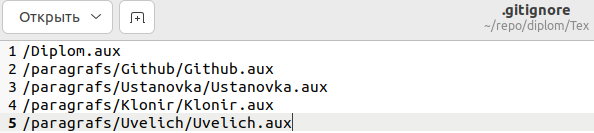
\includegraphics[width=0.6\linewidth]{VM/gitignore.png}
\caption{Файл .gitignore с списком файлов для игнорирования в нём.}
\label{ris:image}
\end{figure}

Это не единственный способ задания игнорирования файла или каталога. Можно также сообщить Git всегда игнорировать определенные файлы во всех репозиториях на компьютере. Для этого, например, каталог нужно добавить в файл с именем ignore , расположенным внутри каталога \texttt{~/.config/git}.

Также можно вообще не создавать файл .gitignore. Этот метод можно использовать для локально создаваемых файлов, которые не должны создавать другие пользователи. Для этого, используя текстовый редактор, нужно открыть файл, вызываемый \texttt{.git/info/exclude} в корневом каталоге репозитория Git.